\documentclass[twocolumn]{revtex4}
\usepackage{amssymb}
\usepackage{amsmath}
\usepackage{amsfonts}
\usepackage{graphicx}
\usepackage{float}
%\usepackage{forloop}
\usepackage{tikz}
\usepackage{mhchem}

\begin{document}

\title{Intrinsic Variables and State Reconstruction in Multiscale Simulations}

%\author{}
%\email{}
%\affiliation{}

\date{\today}

\begin{abstract}
Finding informative low-dimensional descriptions of high dimensional simulation data
(like the ones arising in Molecular Dynamics or kinetic Monte Carlo simulations of
physical/chemical processes) is crucial in understanding physical phenomena, and can
also dramatically assist in accelerating the simulations themselves.
%
In this paper we discuss and illustrate the use of nonlinear intrinsic variables (NIVs)
in the mining of high-dimensional multiscale simulation data.
%
In particular we focus on the way that NIVs allow us to functionally merge different
simulation ensembles, and {\em different partial observations of these ensembles}, as well
as to infer variables not explicitly observed/measured.
%
The approach relies on certain simple features of the underlying process variability to
filter out measurement noise and systematically recover a unique reference coordinate frame.
%
We illustrate the approach through two distinct sets of multiscale atomistic simulations: a fast/slow
time scale Stochastic Simulation Algorithm simulation of enzyme kinetics, and a molecular
dynamics simulation of alanine dipeptide in explicit water.

\end{abstract}

\keywords{Intrinsic variables, partial observations, complex dynamical systems}

\maketitle

\section{Introduction}
The last decade has witnessed extensive advances in dimensionality reduction techniques:
finding meaningful low-dimensional descriptions of high-dimensional data.
%
These developments have the potential to significantly enable the computational exploration
of phyiscochemical problems.
%
If the (high-dimensional) data $Y(t)$ arise from, say, a
molecular dynamics simulation of a macromolecule in solution, or from the stochastic
simulation of a complex chemical reaction scheme, the detection of a few good, coarse-grained
``reduction coordinates" $x(t)$ is invaluable in understanding/predicting system behavior.
%
enhancing, acceleration...

%
While the benefits from such reduced descriptions are manifest, a crucial shortcoming of
such data-driven reduction coordinates is their dependence on the specific data set processed,
and not only on the physical model in question.
%
It is well known that, even in the simple linear case of Principal Component Analysis,
different data sets on the same low-dimensional hyperplane in the ambient space $Y$
will lead to different basis vectors spanning it - in effect, to different $x$.
%
And while this can be easily fixed by a linear transformation, the problem becomes
exacerbated when the low-dimensional space is curved (a manifold, rather than a hyperplane)
and when different data ensembles are obtained using different instrumental modalities
(say, when one wants to merge molecular dynamics data with spectral information).
%
Clearly, the ability to systematically construct a {\em unique, consistent} reduction
coordinate set, shared by all different measurement ensembles and observation modalities -
what we call a (Nonlinear) Intrinsic Variable Set, is invaluable.
%
Embedding in such a coordinate set allows us to naturally merge different observations of the same system;
more importantly, it enables the construction of an empirical mapping between these different
observation ensembles, allowing us to complete partial measurements through the construction
of nonlinear observers of unmeasured variables.
%
This latter empirical mapping requires good interpolation tools in embedding space; to this
end we will demonstrate here the use of a multiscale Laplacian Pyramid approach \cite{rabin2012heterogeneous}.
%
We chose two distinct multiscale illustrative examples. The first is a Gillespie Stochastic Simulation
Algorithm (SSA)  of two Goldbeter-Koshland modules in an enzyme kinetics model \cite{zagaris2012stability}; separation of time scales is known,
in certain parameter regimes, to reduce this model to a two-dimensional effective description.
The second example is the molecular dynamics
simulation (in explicit water) of a simple peptide fragment (alanine dipeptide) whose folding
dynamics are known to be described through a small set of physical observables (two dihedral angles).
%
The paper is structured as follows: in Section \ref{sec:NIV} we present Nonlinear Intrinsic Variable formulation and
the associated inference method. Section \ref{sec:LapPyr} contains our discussion of Laplacian Pyramids that
will be used for the completion of partial observations. Section \ref{sec:examples} contain the results
of applying the approach to simulation data from our two illustrative examples. We conclude with
a summary and discussion of open issues in Section \ref{sec:conclusions}.

\section{Nonlinear Intrinsic Variables} \label{sec:NIV}

\begin{figure*}[ht]
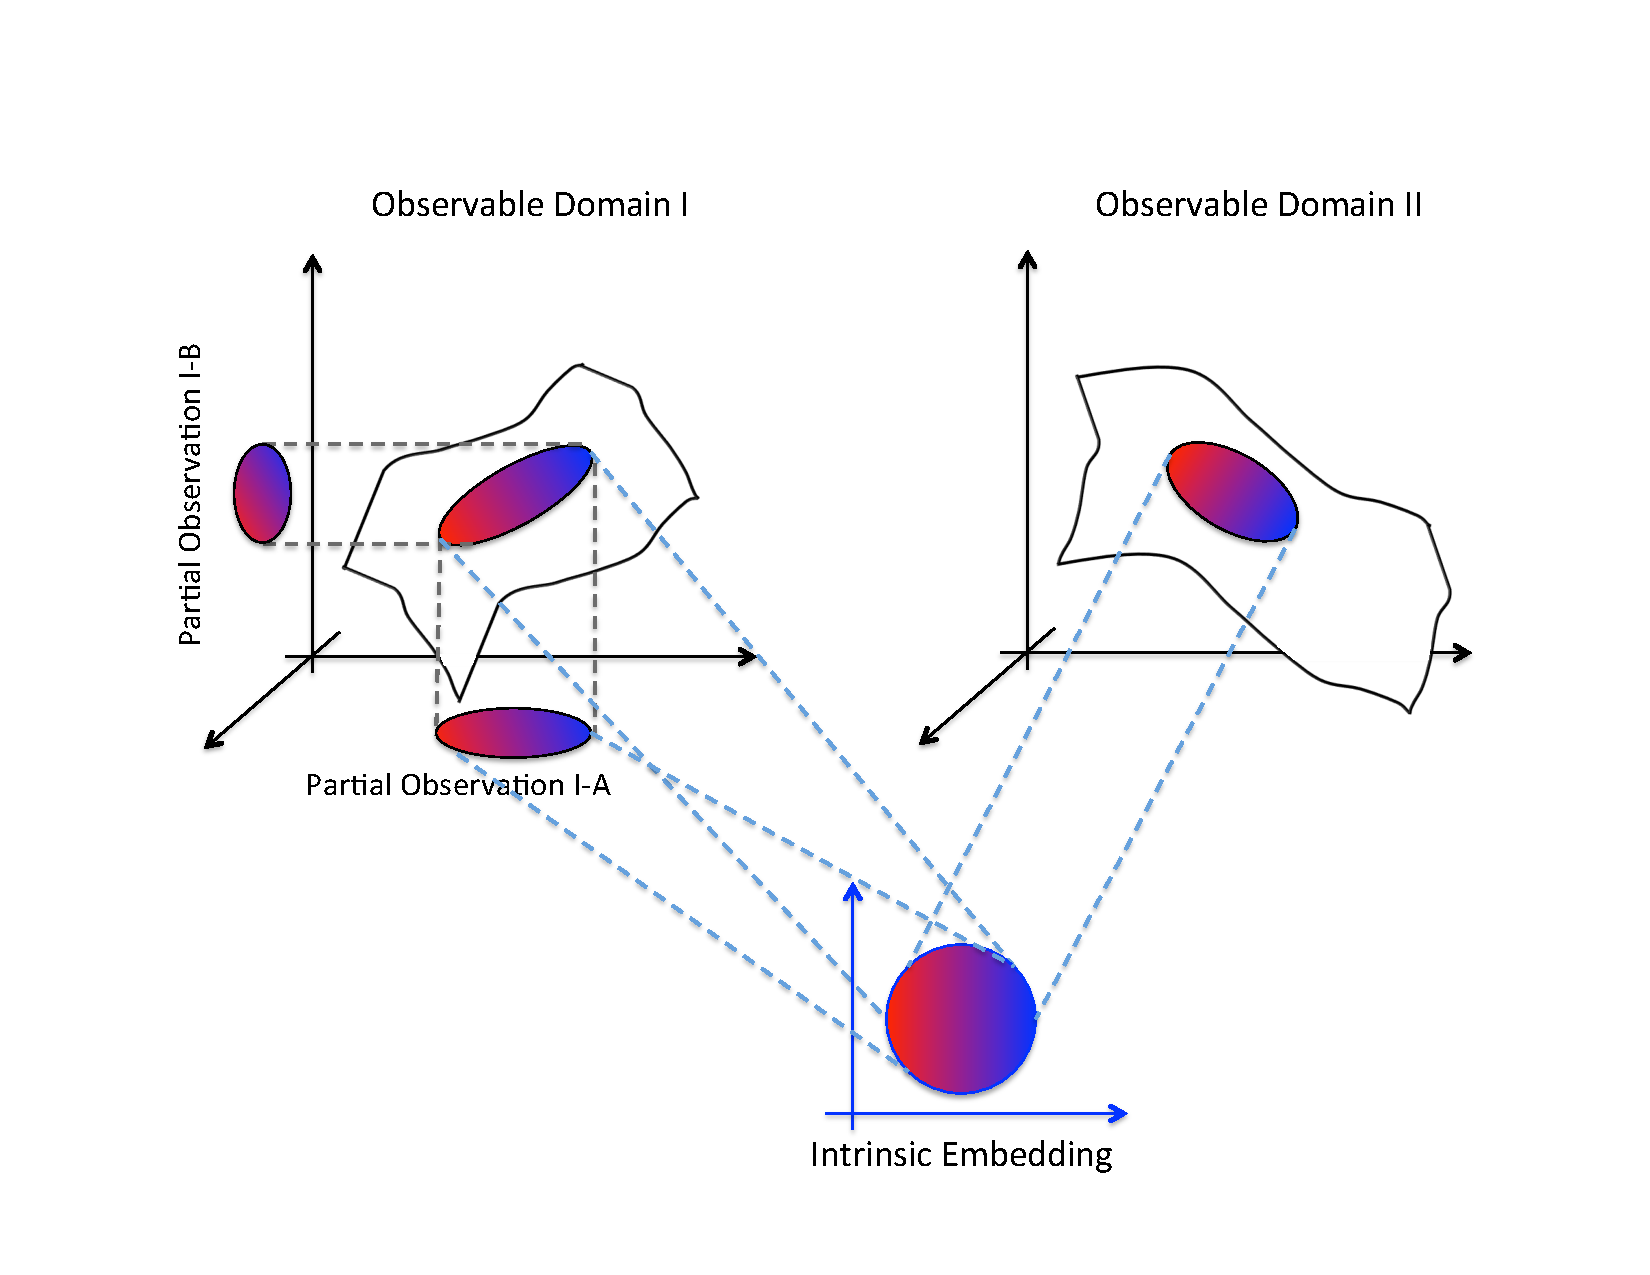
\includegraphics[width=0.7\textwidth]{IntrinsicEmbeddingIllustration2.pdf}
\caption{Illustration of the nonlinear embedding that yields an intrinsic representation independent of measurement modality. (Bottom) The underlying variables in which the diffusion parameters are independent with unit variance. The circle illustrates the end points of the short bursts that create a sphere around the initial point on the manifold. (Top Lft) The first set of observed variables. The ellipse illustrates the end points of the short bursts as observed via the first observation modality. (Top right) The second set of observed variables. The ellipse illustrates the end points of the short bursts as observed via the second observation modality.}
\end{figure*}

{\bf To do:} \\
Block diagram/algorithm

\section{Laplacian Pyramids} \label{sec:LapPyr}

{\bf To do:} \\
A flow chart/block diagram of the method (possibly with the formulas).\\
Maybe an illustration of the multiscale reconstruction of functions.

\begin{figure*}[ht]
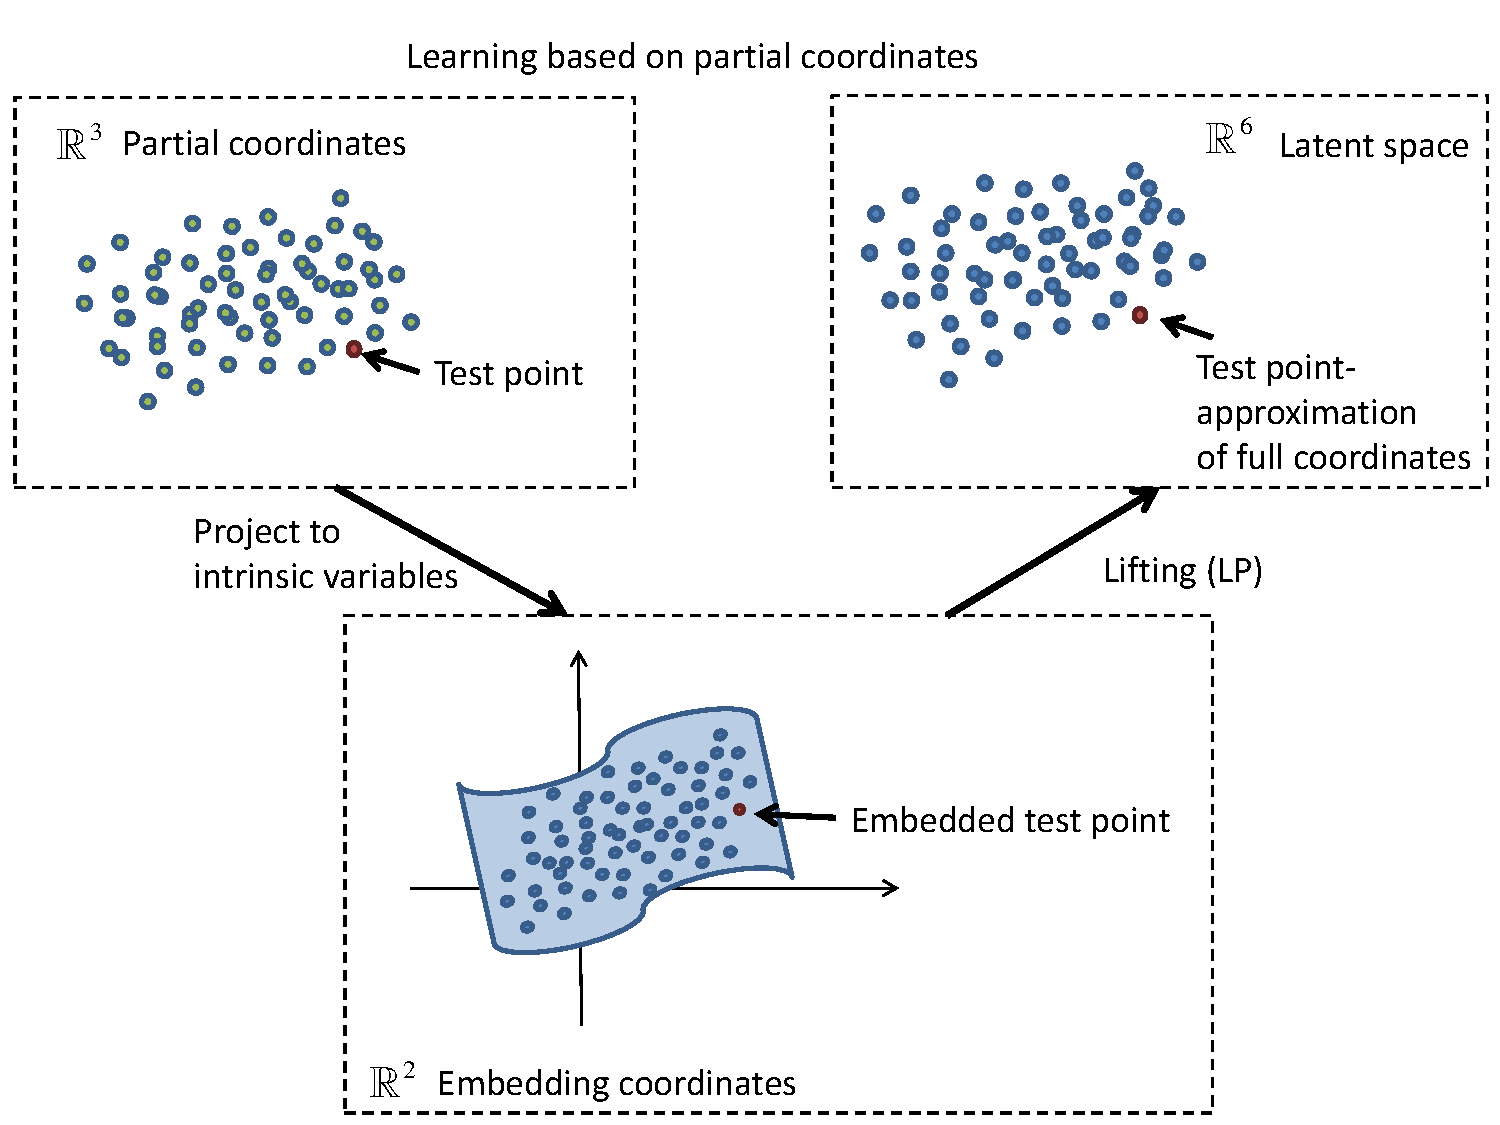
\includegraphics[width=0.7\textwidth]{LapPyr_illustration.pdf}
\caption{Illustration of overall methodology}
\end{figure*}

\section{Models and Results} \label{sec:examples}

\subsection{Chemical Reaction Network}

We first consider a chemical reaction network of multiple enzyme-substrate interactions \cite{zagaris2012stability}.
%
The equations that govern the network are\\
\begin{center}
\ce{$E$ + $S$ <=>[e_1][e_{-1}] $E:S$ ->[e_2][] $E$ + $S^{*}$}\\
\ce{$S$ + $E$ <=>[b_1][b_{-1}] $S:E$ ->[b_2][] $S$ + $E^{*}$}\\
\ce{$D$ + $S^{*}$ <=>[d_1][d_{-1}] $D:S^{*}$ ->[d_2][] $D$ + $S$}\\
\ce{$F$ + $E^{*}$ <=>[f_1][f_{-1}] $F:E^{*}$ ->[f_2][] $F$ + $E$}\\
\end{center}

The $^{*}$ denote activated forms of the various species, and the : denote complexes formed between two species; the complexes $E:S$ and $S:E$ are not equivalent.

There are 10 species in this reaction system.
%
However, one can write four conservation equations (since total $E$, $S$, $D$, and $F$ are all conserved) to reduce the system to 6 dimensions.
%
We assume each reaction follows an elementary rate law.
%
We use the parameters $b_1=5$, $d_1=0.0009$, $e_1=0.1$, $f_1=0.1$, $b_{-1} = 10.6$, $d_{-1}=0.05$, $e_{-1}=0.5$, $f_{-1} =0.01$, $b_2=0.4$, $d_2=0.85$, $e_2=0.05$, and $f_2=2$.
%
We take $S_T=E_T=D_T=1$, and $F_T=0.02$, where $S_T$, $E_T$, $D_T$, and $F_T$ are total concentrations of $S$, $E$, $D$, and $F$, respectively.
%
In this parameter regime, the system exhibits a separation of timescales, so that initial conditions quickly approach a two-dimensional manifold.
%
%The relevant timescales around the steady state ($-1/\lambda_i$, where $\lambda_i$ are the eigenvalues of the Hessian) are 1176, 9.731, 1.594, 1.111, 0.4975, 0.06498.

Although chemical reaction systems are typically thought of as governed by a system of ODEs, the ODEs are only an approximation that holds in the limit of a large number of molecules.
%
When the number of molecules is small, the system is inherently stochastic and its dynamics can be simulated using the Gillespie Stochastic Simulation Algorithm (SSA) \cite{gillespie1977exact}.
%
We can control the level of noise in the system by adjusting the volume $V$ (and therefore adjusting the number of molecules); in our simulations, we take $V=10^5$.
%
The volume is small enough so that we can still see appreciable stochasticity in small simulation bursts, but large enough so that the underlying two-dimensional manifold is (relatively) smooth.

We generate 3000 random initial conditions (enforcing that all concentrations must be non-negative),
and then integrate each point forward for 10 time units using the Gillespie algorithm.
%
10 time units is sufficiently long for the initial points to converge to the two-dimensional manifold,
but not long enough for the points to converge to the final steady state or to a one-dimensional curve.
%
We take these final points to be representative of points on the manifold; three-dimensional projections of the resulting manifold are shown in Figure \ref{fig:rxn_manifolds}.
%
From each manifold point, we run 20 short simulations, each for 0.2 time units.
%
We then use these short simulation ``bursts'' to estimate the local covariances for NIV.

\begin{figure*}[ht]
  \includegraphics[height=6cm]{rxn_figures/rxn_manifold1.jpg}\llap{\raisebox{3.5cm}{\includegraphics[height=2.5cm]{rxn_figures/rxn_manifold1_2.jpg}}}
  \includegraphics[height=6cm]{rxn_figures/rxn_manifold2.jpg}\llap{\raisebox{3.5cm}{\includegraphics[height=2.5cm]{rxn_figures/rxn_manifold2_2.jpg}}} \\
  \includegraphics[height=6cm]{rxn_figures/rxn_manifold3.jpg}\llap{\raisebox{3.5cm}{\includegraphics[height=2.5cm]{rxn_figures/rxn_manifold3_2.jpg}}}
  \includegraphics[height=6cm]{rxn_figures/rxn_manifold4.jpg}\llap{\raisebox{3.5cm}{\includegraphics[height=2.5cm]{rxn_figures/rxn_manifold4_2.jpg}}} \\
    \caption{Projections of the manifold from stochastic simulation of the chemical reaction network. The insets show rotations of the projections to illustrate the two-dimensionality of the manifold.}
    \label{fig:rxn_manifolds}
\end{figure*}

We consider two different data sets from our simulations.
%
In data set 1, we only observe components $E$, $S$, $S:E$, and $F:E^{*}$; in data set 2, we only observe components $E$, $S$, $E:S$, and $D:S^{*}$.
%
We wish to use NIV together with Laplacian Pyramids to predict the values of $S:E$ and $F:E^{*}$ in data set 2.

Figure \ref{fig:rxn_embedding} shows the two-dimensional NIV embeddings for the two different data sets; the embeddings appear very consistent.
%
In addition, the two data sets contain 500 common data points.
%
We use these data points to compute the correlation between the embeddings for data set 1 and data set 2.
%
We obtain a correlation of 0.97 and 0.95 between the two data sets for the first and second NIVs, respectively, indicating that the two embeddings are in excellent agreement with each other.

\begin{figure*}[ht]
    \includegraphics[width=0.4\textwidth]{rxn_figures/rxn_NLICA1.jpg}
    \includegraphics[width=0.4\textwidth]{rxn_figures/rxn_NLICA2.jpg}
    \includegraphics[width=0.4\textwidth]{rxn_figures/rxn_NLICA_corr1.jpg}
    \includegraphics[width=0.4\textwidth]{rxn_figures/rxn_NLICA_corr2.jpg}
    \caption{(Top, left) NIV embedding obtained from data set 1 (observations of components E, S, S:E, and F:E$^{*}$), colored by $S$. (Top, right) NIV embedding obtained from data set 2 (observations of components E, S, E:S, and D:S$^{*}$), colored by $S$. (Bottom, left) Correlation of first NIV between two different embeddings (correlation=0.97). (Bottom, right)  Correlation of second NIV between two different embeddings (correlation=0.95).}
    \label{fig:rxn_embedding}
\end{figure*}

We then use Laplacian Pyramids to predict $S:E$ and $F:E^{*}$ in data set 2.
%
Because data set 1 and data set 2 are measured for different components, there is no simple way to estimate $S:E$ and $F:E^{*}$ from the two data sets in the observation space.
%
Instead, we must first project the data into the NIV space so that we can compute neighbors {\em between} the two data sets.
%
We use data set 1 to train a Laplacian Pyramids function from the two-dimensional NIV embedding to $S:E$ and $F:E^{*}$.
%
We then use this function to predict the values  of $S:E$ and $F:E^{*}$ for data set 2, using the computed NIV embedding for data set 2.
%
In this way, we are exploiting the fact that the NIV embedding is intrinsic and consistent between the two data sets, even though the two data sets contain measurements of different components.
%
The results of the Laplacian Pyramids prediction are seen in Figure \ref{fig:rxn_recon}.
%
The MSE between the true and predicted values is .....

\begin{figure*}[ht]
    \includegraphics[width=0.4\textwidth]{rxn_figures/chm4_from_Em.png}
    \includegraphics[width=0.4\textwidth]{rxn_figures/chm6_from_Em.png}
    \caption{Laplacian Pyramids (LapPyr) and nearest neighbor (nn) reconstructions of $S:E$ (left) and $F:E^{*}$ (right).}
    \label{fig:rxn_recon}
\end{figure*}

\subsection{Alanine Dipeptide}

Our second example comes from a simulation of a small peptide fragment.
%
Alanine dipeptide (Ala2) is often used as a ``prototypical'' protein for simulation studies.
%
We simulate the motion of Ala2 in explicit solvent using the AMBER 10 molecular simulation package \cite{case2008Amber} with an
optimized version \cite{best2009optimized} of the AMBER ff03 force field \cite{duan2003point}.
%
The molecule was solvated with 638 TIP3P water molecules \cite{jorgensen1983comparison}, with the particle mesh Ewald method used for long-range electrostatic interactions \cite{essmann1995smooth} and periodic boundary conditions.
%
The simulation is performed at constant volume and temperature (the NVT ensemble), with the temperature being maintained at 300~K with a Langevin thermostat \cite{loncharich1992langevin}.
%
Hydrogen bonds were fixed using the SHAKE algorithm \cite{ryckaert1977numerical}.
%
The two dihedral angles $\phi$ and $\psi$ are known to parameterize the free energy surface, and the free energy surface contains three minima (labeled A, B, and C, see Figure \ref{fig:ala_fes}).
%
Our simulations were concentrated around minimum B in the free energy surface, located at $\phi=-65^{\circ}$, $\psi=150^{\circ}$.
%
We start many simulations at $10^{\circ}$ away from the minimum, and allow the simulations to each run for 0.1~ps; we record the configuration every 1~fs.
%
Configurations are stored with all atoms except the hydrogens.

\begin{figure*}[ht]
    \includegraphics[width=0.6\textwidth]{FES.pdf}
    \includegraphics[width=0.3\textwidth]{molecule_labeled2.jpg}
    \caption{(Left) Free energy surface for Alanine Dipeptide. The minima are labeled A, B, and C, and the corresponding molecular configurations are shown. (Right) The molecular structure of alanine dipeptide, excluding the hydrogens. The atoms are numbered and the two dihedral angles $\phi$ and $\psi$ are indicated.}
    \label{fig:ala_fes}
\end{figure*}


We first wish to demonstrate the benefit of NIV over other nonlinear dimensionality reduction techniques, such as diffusion maps.
%
We compute the NIV embedding for 10,000 data points using only atoms 2, 4, 6, 8, and 10.
%
We then compute the NIV embedding for the same 10,000 data points using only atoms 5, 7, and 9.
%
We also do the same using diffusion maps instead of NIV.
%
The correlation between the NIV coordinates for the two data sets and the diffusion maps coordinates for the two data sets are shown in Figure \ref{fig:ala_corr}.
%
The correlation between the two NIV embeddings is higher than the correlation between the two diffusion maps embeddings.

\begin{figure*}[ht]
    \includegraphics[width=0.4\textwidth]{ala_figures_evenodd/NLICA_corr.jpg}
    \includegraphics[width=0.4\textwidth]{ala_figures_evenodd/DM_corr.jpg}
    \caption{Correlation between the second NIV (left) and the second DM (right) computed using the atoms 5, 7, and 9 and using the atoms 2, 4, 6, 8, and 10.}
    \label{fig:ala_corr}
\end{figure*}

\begin{table}
\begin{tabular}{| r || c | c |}
  \hline
  & Coordinate 1 & Coordinate 2 \\
  \hline
  \hline
  NLICA & 0.62 & 0.84 \\
  \hline
  DM & 0.54 & 0.60 \\
  \hline
\end{tabular}
\caption{Correlation between the embedding coordinates from NLICA and DMAPS using the atoms 5, 7, and 9 and using the atoms 2, 4, 6, 8, and 10.}
\end{table}

We then use NIV together with Laplacian Pyramids to predict the conformation of Ala2 when we only observe some of the atoms.
%
Our training data consists of 10,000 data points, each containing the coordinates of all the atoms in Ala2.
%
We compute the NIV embedding for the training data, and then train Laplacian Pyramids to go from the NIV embedding to the moelcular configuration.
%
The NIV embedding for the training data is shown in Figure \ref{fig:ala_embed}.
%
The embedding is three-dimensional; the first coordinate describes the flipping of atoms 1 and 3, the second coordinate describes the dihedral angle $\phi$, and the third coordinate describes the dihedral angle $\psi$.

We then take 12,000 test data points.
%
Each test point contains the coordinates of {\em only} the odd atoms in Ala2.
%
2,000 of the test points are also contained in the training data set, so that we can evaluate the consistency of the two embeddings.
%
We compute the NIV embedding for the test data points, and then use the Laplacian Pyramids from the training data to predict the location of all the atoms for each point in the test data.

\begin{table}
\begin{tabular}{| r || c | c | c |}
  \hline
  & Coordinate 1 & Coordinate 2 & Coordinate 3 \\
  \hline
  \hline
  NLICA & 0.97 & 0.72 & 0.85 \\
  \hline
  DM & 0.95 & 0.76 & 0.74 \\
  \hline
\end{tabular}
\caption{Correlation between the embedding coordinates from NLICA and DMAPS using all and just odd coordinates.}
\end{table}

\begin{figure*}[ht]
    \includegraphics[width=0.3\textwidth]{ala_figures_allodd/ala2_embed1.jpg}
    \includegraphics[width=0.3\textwidth]{ala_figures_allodd/ala2_embed2.jpg}
    \includegraphics[width=0.3\textwidth]{ala_figures_allodd/ala2_embed3.jpg}
    \caption{The 3-dimensional NIV embedding for Alanine Dipeptide computed using all the atoms, colored by the y-coordinate of the first atom (left), the dihedral angle $\phi$ (center), and the dihedral angle $\psi$ (right). Each embedding is rotated so that the correlation between the colors and the relevant NIV can easily be seen.}
    \label{fig:ala_embed}
\end{figure*}

The embeddings for the two data sets are found to be fairly consistent, with correlations of 0.97, 0.72, 0.85 for the first, second, and third NIVs, respectively.
%
Figure \ref{fig:ala_recon} shows the reconstructed position versus true position for some selected atoms.
%
The atoms that have significant movement (such as atoms 1 and 3) exhibit a strong correlation between the true and reconstructed positions.
%
Figure \ref{fig:ala_molecules} shows molecular structures for the true and reconstructed configurations for some data points.
%
There is nice agreement between the true and reconstructed configurations.

\begin{figure*}[ht]
  \centering
    \foreach \atomnumber in {1,2,3,6,8} {
        \includegraphics[width=0.2\textwidth]{ala_figures_allodd/ala2_recon_corr_\atomnumber_1.jpg}
        \includegraphics[width=0.2\textwidth]{ala_figures_allodd/ala2_recon_corr_\atomnumber_2.jpg}
        \includegraphics[width=0.2\textwidth]{ala_figures_allodd/ala2_recon_corr_\atomnumber_3.jpg}\\
      }
  \caption{The correlation between the true position and the reconstructed position (using Laplacian Pyramids) for the test data. The columns correspond the x-, y-, and z-coordinates, and the rows correspond to atoms 1, 2, 3, 6, and 8.}
  \label{fig:ala_recon}
\end{figure*}

\begin{figure*}[ht]
    \centering
    \includegraphics[width=0.3\textwidth,trim=0.5in 3in 4in 0.5in, clip]{molec_figures/molecule300_balls.jpg}
    \includegraphics[width=0.3\textwidth,trim=0.5in 3in 4in 0.5in, clip]{molec_figures/molecule300_wire.jpg}\\
    \includegraphics[width=0.3\textwidth,trim=0.5in 3in 4in 0.5in, clip]{molec_figures/molecule600_balls.jpg}
    \includegraphics[width=0.3\textwidth,trim=0.5in 3in 4in 0.5in, clip]{molec_figures/molecule600_wire.jpg}\\
    \includegraphics[width=0.3\textwidth,trim=0.5in 3in 4in 0.5in, clip]{molec_figures/molecule900_balls.jpg}
    \includegraphics[width=0.3\textwidth,trim=0.5in 3in 4in 0.5in, clip]{molec_figures/molecule900_wire.jpg}
    \caption{True structure (black) and reconstructed structure (red) for three different data points. Each data point is shown in ``ball-and-stick'' representation (left) and ``wireframe'' representation (right) so that the discrepancies can easily be seen between the different configurations.}
    \label{fig:ala_molecules}
\end{figure*}

\section{Conclusions} \label{sec:conclusions}

\begin{acknowledgments}
The authors would like to thank...
\end{acknowledgments}

\bibliography{../../references/references}

\appendix

\section{Chemical Reaction Network Parameters}
The reaction network
\begin{center}
\ce{$E$ + $S$ <=>[e_1][e_{-1}] $E:S$ ->[e_2][] $E$ + $S^{*}$}\\
\ce{$S$ + $E$ <=>[b_1][b_{-1}] $S:E$ ->[b_2][] $S$ + $E^{*}$}\\
\ce{$D$ + $S^{*}$ <=>[d_1][d_{-1}] $D:S^{*}$ ->[d_2][] $D$ + $S$}\\
\ce{$F$ + $E^{*}$ <=>[f_1][f_{-1}] $F:E^{*}$ ->[f_2][] $F$ + $E$}\\
\end{center}

is governed by the following ODEs
\begin{equation}
    \begin{array}{rcl}
        \frac{d S}{dt} & = & -e_1 S E + e_{-1} E:S -b_1 S E \\
                        &   & + b_{-1} S:E + b_2 S:E + d_2 D:S^{*} \\
        \frac{d E}{dt} & = & -e_1 S E + e_{-1} E:S + e_2 E:S \\
                        &   & - b_1 S E +b_{-1} S:E + f_2 F:E^{*} \\
        \frac{d E:S}{dt}  & = & e_1 S E -e_{-1} E:S -e_2 E:S \\
        \frac{d S:E}{dt}& = & b_1 S E -b_{-1} S:E -b_2 S:E \\
        \frac{d S^{*}}{dt} & = & e_2 E:S -d_1 D S^{*} + d_{-1} D:S^{*} \\
        \frac{d E^{*}}{dt} & = & b_2 S:E -f_1 F E^{*} + d_{-1} F:E^{*} \\
        \frac{d D}{dt} & = & -d_1 D S^{*} + d_{-1} D:S^{*} + d_2 D:S^{*} \\
        \frac{dF}{dt} & = & -f_1 F E^{*} + f_{-1} F:E^{*} + f_2 F:E^{*} \\
        \frac{d D:S^{*}}{dt} & = & d_1 D S^{*} - d_{-1} D:S^{*} -d_2 D:S^{*} \\
        \frac{d F:E^{*}}{dt} & = & f_1 FE^{*} - f_{-1} F:E^{*} -f_2 F:E^{*}
    \end{array}
\end{equation}

We can write four balance equations 
\begin{equation}
    \begin{array}{rcl}
        S_T & = & S^{*} + S + E:S + S:E + D:S^{*} \\
        E_T & = & E^{*} + E + E:S + S:E + F:E^{*} \\
        D_T & = & D + D:S^{*} \\
        F_T & = & F + F:E^{*} 
    \end{array}
\end{equation}

We eliminate $S^{*}$, $E^{*}$, $D$, and $F$ from the system of ODEs.
%
We therefore obtain
\begin{equation}
    \begin{array}{rcl}
        \frac{d S}{dt} & = & -e_1 S E + e_{-1} E:S -b_1 S E \\
                        &   & + b_{-1} S:E + b_2 S:E + d_2 D:S^{*} \\
        \frac{d E}{dt} & = & -e_1 S E + e_{-1} E:S + e_2 E:S \\
                        &   & - b_1 S E +b_{-1} S:E + f_2 F:E^{*} \\
        \frac{d E:S}{dt}  & = & e_1 S E -e_{-1} E:S -e_2 E:S \\
        \frac{d S:E}{dt}& = & b_1 S E -b_{-1} S:E -b_2 S:E \\
        \frac{d D:S^{*}}{dt} & = & d_1 (D_T - D:S^{*}) (S_T - S - E:S - S:E - D:S^{*}) \\
                            &   & - d_{-1} D:S^{*} -d_2 D:S^{*} \\
        \frac{d F:E^{*}}{dt} & = & f_1 (F_T - F:E^{*}) (E_T - E - E:S - S:E - F:E^{*}) \\
                            &   & - f_{-1} F:E^{*} -f_2 F:E^{*}
    \end{array}
\end{equation}

Alternatively, we can write the rates for the 12 chemical reactions as
\begin{equation}
    \begin{array}{rcl}
        r_1 & = & e_1 S E \\
        r_2 & = & e_{-1} E:S \\
        r_3 & = & e_2 E:S \\
        r_4 & = & b_1 S E \\
        r_5 & = & b_{-1} S:E \\
        r_6 & = & b_2 S:E \\
        r_7 & = & d_1 (D_T - D:S^{*}) (S_T - S - E:S - S:E - D:S^{*}) \\
        r_8 & = & d_{-1} D:S^{*} \\
        r_9 & = & d_2 D:S^{*} \\
        r_{10} & = & f_1 (F_T - F:E^{*}) (E_T - E - E:S - S:E - F:E^{*}) \\
        r_{11} & = & f_{-1} F:E^{*} \\
        r_{12} & = & f_2 F:E^{*}
    \end{array}
\end{equation}

For the Gillespie SSA, we use these rates to adjust the {\em number} of each molecule, depending on which reaction occurs.
%
We use the parameters $b_1=5/V$, $d_1=0.0009/V$, $e_1=0.1/V$, $f_1=0.1/V$, $b_{-1} = 10.6$, $d_{-1}=0.05$, $e_{-1}=0.5$, $f_{-1} =0.01$, $b_2=0.4$, $d_2=0.85$, $e_2=0.05$, and $f_2=2$.
%
We take $S_T=E_T=D_T=1V$, and $F_T=0.02V$, where $S_T$, $E_T$, $D_T$, and $F_T$ are total number of $S$, $E$, $D$, and $F$, respectively.
        
\end{document}
